\subsection{Barrier Forming with Minimum Number of Line Segments}

\begin{figure}[ht]
    \centering
    \vspace{.05in}
    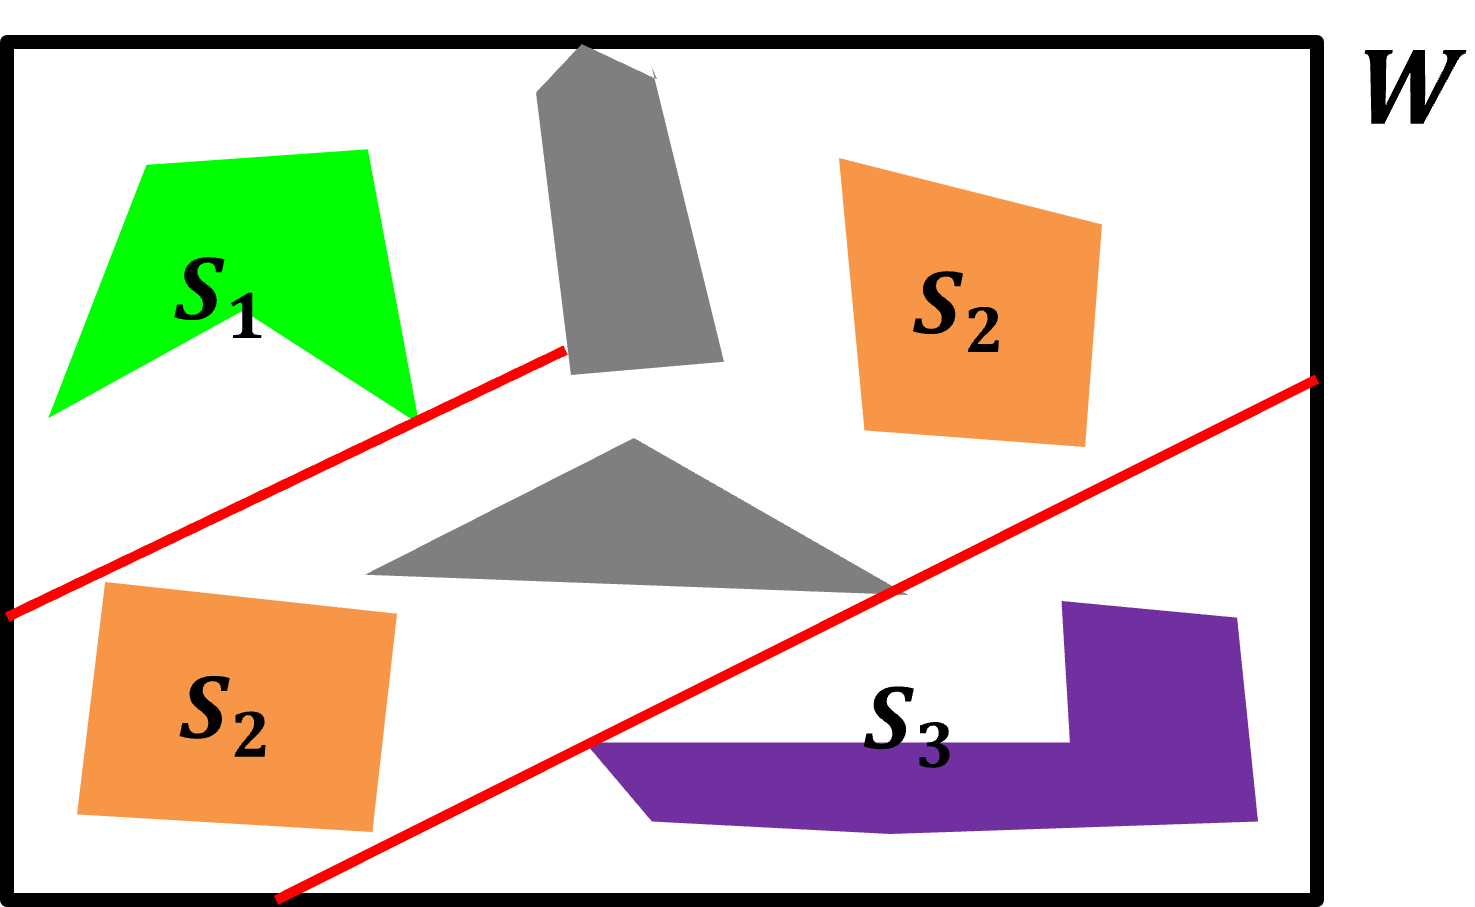
\includegraphics[width = .35\textwidth]{chapters/bf/fig/formulation_pic.png}
    \vspace{.05in}
    \caption{Illustration of a barrier forming problem for the three sets of (colored) polygonal objects $S_{1\sim3}$ among (gray) obstacles. 
    For the setting, $2$ straight lines are sufficient to cut off path connections between any pair of polygon regions from two different sets. 
    In this work, our general goal is to build such barriers with the least number of line segments.}
    \label{fig:bf-illustration}
    % \vspace{-0.2in}
\end{figure}

Let $\mathcal{W}$ be a simply connected polygonal workspace in $\mathbb R^2$. Consider $k$ sets of objects $S_1, \dots, S_k$ in $\mathcal W$, as well as a set of polygonal obstacles $\mathcal O$. 
We seek to use a set of straight line segments $L$ to separate $S_1, \dots, S_k$ from each other, such that for any two objects $o_1 \in S_i$ and $o_2 \in S_j, i \ne j$, any path between $o_1$ and $o_2$ in the free space of $\mathcal W$ must be ``cut off'' by one or more line segments from $L$. 
The line segments do not have length limit and can cross each other, but they cannot cross objects or obstacles in the workspace. We want to find the minimum number of line segments to complete the separation task. 

Under the general formulation of Barrier Forming, we examine three different variants with increasing difficulty:
\begin{enumerate} 
\item \emph{Barriers for point sets}, in which  $S_1, \dots, S_k$ as well as $O$ are sets of points. 
\item \emph{Barriers for point sets among polygonal obstacles}, in which  $S_1, \dots, S_k$ are sets of points but $O$ is a set of polygonal objects. 
\item \emph{Barriers for polygonal objects}, in which $S_1, \dots, S_k$ as well as $O$ contain polygonal objects. 
\end{enumerate}
%The first problem considers points sets for separation, that in this case, $S_1, %\dots, S_k$ are point sets, and there are no obstacles in the workspace. This is the %same as the point set separation problem in the plane. 
%The second still takes $S_1, \dots, S_k$ as point set, but introduces polygonal obstacle sets $\mathcal O$ in the workspace. 
%The last one further considers $S_1, \dots, S_k$ as polygonal object sets.

\subsection{Computational Intractability}
Because the separation of even two sets of points in the plane, 
a special case of the first variant of our barrier forming problem, 
is computationally intractable \cite{demaine2005separating}, 
our first formulation is also NP-hard. 
From here, we can reduce from the first variant to other variants involving polygonal shapes by converting each point object to a sufficiently small polygon. Therefore, all three versions of the barrier forming problems studied in this paper are NP-hard. We omit the straightforward details. 